\documentclass[12pt,letterpaper]{article}

\usepackage[left=1.0in,right=1.0in,top=1.0in,bottom=1.0in,
           includehead=true,headsep=1.0in,includefoot=true]{geometry}
\usepackage{setspace}
\usepackage{url}
\usepackage{tikz}
\usepackage{array}
\usepackage{rotating}
\usetikzlibrary{positioning,shapes,arrows}

\title{
  Clinical Decision Support for OpenMRS
}
\author{
        Bierman, Robert,  \emph{Group Lead}  \\ \texttt{bierman@mail.sfsu.edu} \and 
        Woeltjen, Victor, \emph{Group Lead}  \\ \texttt{woeltjen@mail.sfsu.edu} \and
        Choi, Kay       \and
        Gimeno, Steven  \and
        Lum, Jason      \and
        Ng, Ying Kit    \and
        Uy, Bianca      
} 

\begin{document}


\newpage 

\maketitle
\begin{center}
\begin{Large}\emph{Group 1:} Final Project for CSC 668-868 Spring 2013\end{Large} \linebreak
\url{https://code.google.com/p/sp2013-csc668-868-group1/}
\end{center}
\thispagestyle{empty} % Suppress page number

\newpage \pagenumbering{roman}
\tableofcontents


\newpage \pagenumbering{arabic}
\section{Contributions} 

\subsection{Contributions by Robert Bierman}
Implemented types to represent values in DSS1. Authored Section 
~\ref{sec:INTRODUCTION} of this document. Prepared diagrams, including 
Figures ~\ref{fig:USE_CASE_OVERVIEW} and ~\ref{fig:ARCHITECTURE}.

\subsection{Contributions by Kay Choi}
Added HTML form entry for viral load, CD4, hemoglobin, and 
patient data entry. Added patient summary. Implemented DSS intrinsic read 
functions.

\subsection{Contributions by Steven Gimeno}
Wrote test cases to demonstrate the correctness of the team's implementation 
of the DSS1 language, as seen in Appendix ~\ref{sec:TEST_CASES}.

\subsection{Contributions by Jason Lum}
Implemented DSS intrinsic miscellaneous functions (within, length). 
Authored documentation for intrinsic functions, Section ~\ref{sec:INTRINSIC_FUNCTIONS}. Authored use cases shown in Section ~\ref{sec:USE_CASES}.

\subsection{Contributions by Ying Kit Ng}
Studied the Spring web MVC (Model View Controller) framework to integrate 
the compiler. Implemented the DSSDate intrinsic functions. Prepared screen 
shots for user guide, Section ~\ref{sec:USER_GUIDE}.

\subsection{Contributions by Bianca Uy}
Authored web pages and implemented server-side controllers to create and edit 
DSS rules. Integrated alert functionality for client-side display. Authored 
text of user guide, Section ~\ref{sec:USER_GUIDE}.

\subsection{Contributions by Victor Woeltjen}
Implemented DSS Rule Service, including rule storage and conversion to and from XML (Extensible Markup Language). Implemented flow control, execution 
context, and integrated value types into DSS Interpreter. Authored sections 
~\ref{sec:DESIGN_OVERVIEW} and
~\ref{sec:CLASS_DIAGRAMS} of this document, except for subsections otherwise noted.


\newpage 
\section{Introduction} \label{sec:INTRODUCTION}

\subsection{Problem statement}

It is one thing to have information readily available, it is another to understand and make the best use of that information.  The OpenMRS system provides a repository of data on patients but it is still up to the physician to decide the course of treatment, tests that need to be run, and medications to be administered.  The Decision Support System (DSS) is designed to assist the physician by providing alerts based on correlation of data and programmatic rules.  Because of the vast amounts of data on patients, the number of medications and tests available and the variability of patient behavior, the DSS is designed to provide rules to avoid mistakes, speed patient care and optimize resources.

DSS allows doctors to create rules to alert them if they prescribe a medication that may interact with other medications that the patient is taking or may be allergic to.   Or, it can suggest running tests that may be due or alert to the fact that prior tests need to be redone.  Decision support is about correlating the data is a manner useful to the physician.

To create a DSS, a method must exist to specify these rules, and should be of a nature to allow non-technical individuals to create them.  Once created a system to store and interpret those rules needs to be devised and finally the results of the rules need to be displayed back to the physician in an intuitive and meaningful way.

The task here is given the presented language grammar (see appendix A), create the interpreter that can store and process rules and display the results on the patient summary and dashboards in OpenMRS.

\subsection{Software and platform used}

This solution has been implemented as a module for OpenMRS. The DSS Interpreter has been written in Java. Client pages have been written 
in JavaScript, JSP, and HTML, with OpenMRS extension points indicated using 
XML. Interactions between the web-based client and server-side rules are 
supported by the Spring framework and DWR (Direct Web Remoting).

\begin{figure}\begin{center}
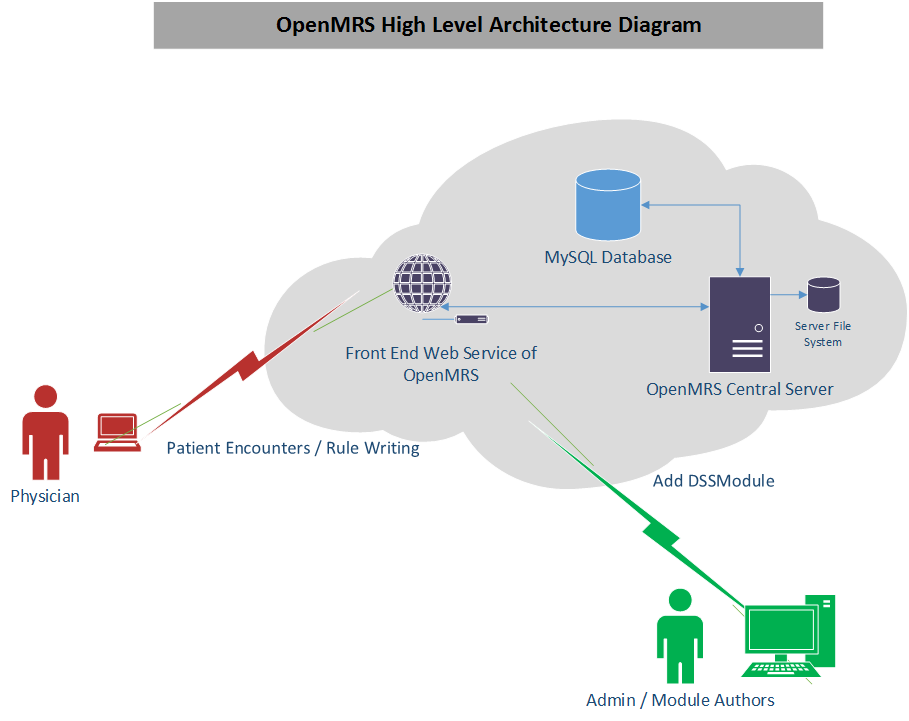
\includegraphics[width=6.5in]{OpenMRS_Architecture.png}
\end{center}
\caption{Architecture Diagram} \label{fig:ARCHITECTURE}
\end{figure}

\newpage 
\section{User guide} \label{sec:USER_GUIDE}

\subsection{First steps}
	Log onto OpenMRS with your corresponding username and password. Passwords are case-sensitive. Once logged in, you can search or create a patient using the tab 'Find/Create Patient'. Once you have selected the patient, their profile will appear.

\subsection{Patient profile}
	Patient profile has several tabs – Overview, Regimens, Visits, Demographics, Graphs, Form Entry, Example, Vitals, and Notes.  There is also a patient summary link and underneath are any alerts that a physician may need to be aware about the patient (Figure ~\ref{fig:PATIENT_PROFILE}).

\begin{figure}\begin{center}
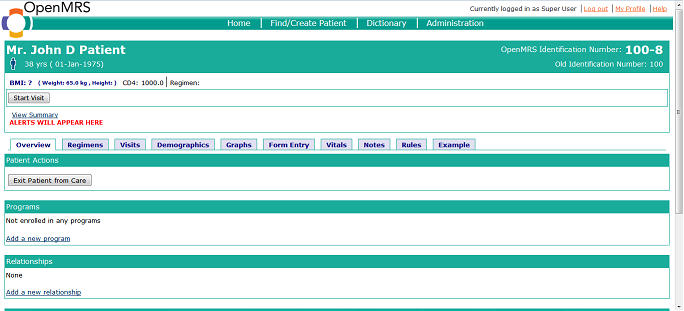
\includegraphics[width=6.5in]{user_guide/patient_profile.png}
\end{center}
\caption{Patient profile}
\label{fig:PATIENT_PROFILE}
\end{figure}

\subsubsection{Form entry}
	There are four different forms available – Vitals, Viral, Hemoglobin, and CD4 (Figure ~\ref{fig:VITALS_FORM}, 
	~\ref{fig:VIRAL_FORM}, ~\ref{fig:HEMOGLOBIN_FORM}, 
	and ~\ref{fig:CD4_FORM}, 
	). Viral, Hemoglobin, and CD4 are for lab results. The encounter details must be filled along with the data entry. The Vitals form is an assessment of the current condition of the patient. Once the form is completed, press “Enter Form” and all information will be saved. 
	The forms from the last three encounters are available for viewing; for a more complete listing, check “Visits” tab.

\begin{figure}\begin{center}
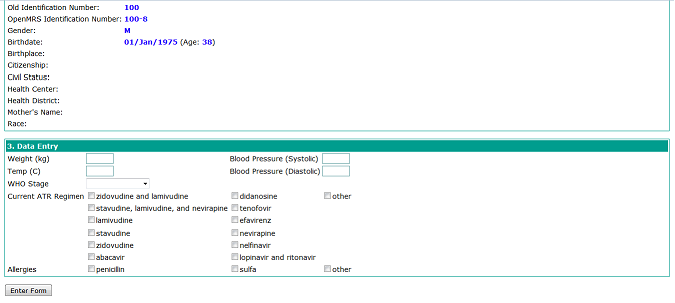
\includegraphics[width=6.5in]{user_guide/vitals_form.png}
\end{center}
\caption{Vitals form}
\label{fig:VITALS_FORM}
\end{figure}

\begin{figure}\begin{center}
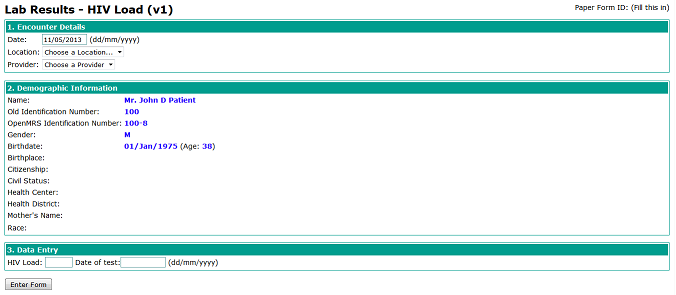
\includegraphics[width=6.5in]{user_guide/viral_form.png}
\end{center}
\caption{Viral form}
\label{fig:VIRAL_FORM}
\end{figure}

\begin{figure}\begin{center}
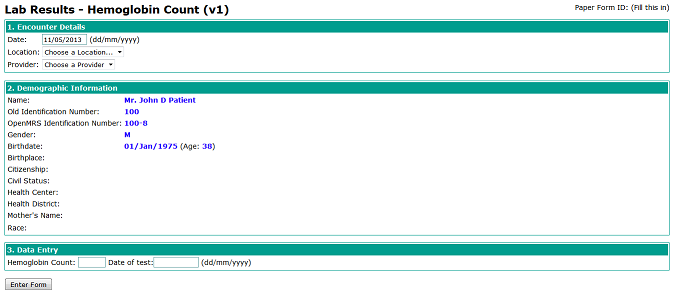
\includegraphics[width=6.5in]{user_guide/hemoglobin_form.png}
\end{center}
\caption{Hemoglobin form}
\label{fig:HEMOGLOBIN_FORM}
\end{figure}

\begin{figure}\begin{center}
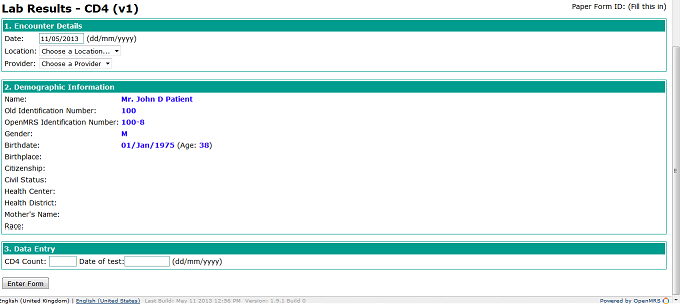
\includegraphics[width=6.5in]{user_guide/cd4_form.png}
\end{center}
\caption{CD4 form}
\label{fig:CD4_FORM}
\end{figure}


\subsubsection{Vitals tab}
	Displays the weight, systolic blood pressure, diastolic blood pressure, and temperature of the patient based the latest encounter without having to pull out the form (Figure ~\ref{fig:VITALS_TAB}).

\begin{figure}\begin{center}
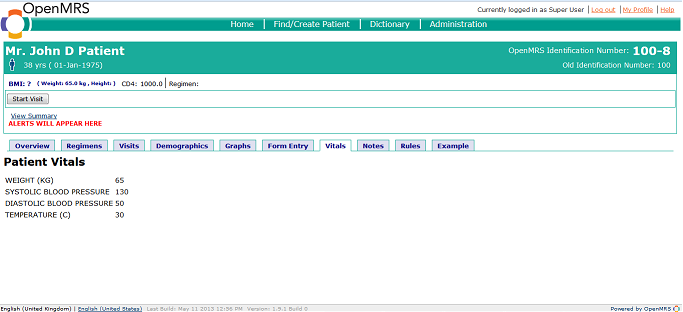
\includegraphics[width=6.5in]{user_guide/vitals_tab.png}
\end{center}
\caption{Vitals tab, displaying weight, blood pressure, and temperature 
based on latest encounter.}
\label{fig:VITALS_TAB}
\end{figure}

\subsubsection{Patient summary}
	Includes allergies, all ART regimen drugs, who stage, and TB status; it also includes the vitals of the patient from the first encounter and the last encounter; and all lab results – viral, hemoglobin, and cd4. Any alerts that a physician may need to be aware of are displayed in the bottom of the page in large bold letters (Figure ~\ref{fig:PATIENT_SUMMARY}). These information are all based on patient encounters.

\begin{figure}\begin{center}
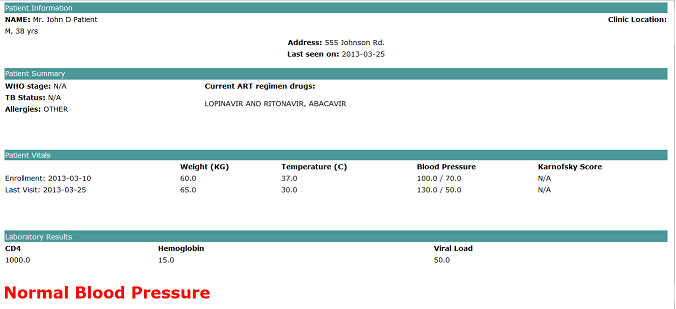
\includegraphics[width=6.5in]{user_guide/patient_summary.png}
\end{center}
\caption{Patient summary}
\label{fig:PATIENT_SUMMARY}
\end{figure}


\subsubsection{Alerts}
	Alerts are generated based on DSS rules on OpenMRS which utilizes information from patient encounters. They can be found in two locations – patient dashboard and patient summary. Figure ~\ref{fig:PATIENT_PROFILE} and ~\ref{fig:PATIENT_SUMMARY} shows where the alerts will appear on the patient dashboard and patient summary, they appear in bold red letters.

\subsection{Administrator}
	Under “Administration” and under the heading “DSS Compiler” there are two links that provides you a way to create new rules onto OpenMRS (Figure 
	~\ref{fig:ADMINISTRATION_PAGE}). Once rules are loaded onto the system, they cannot be deleted. A loading image may appear while the rules are rendering prohibiting you from using the page, it will disappear once it is done.

\begin{figure}\begin{center}
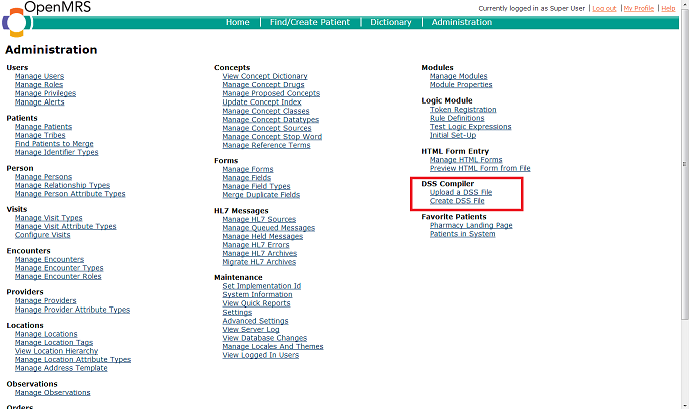
\includegraphics[width=6.5in]{user_guide/administration.png}
\end{center}
\caption{Administration page}
\label{fig:ADMINISTRATION_PAGE}
\end{figure}

\subsubsection{Upload a DSS rule}
	You can upload an existing .DSS file onto OpenMRS. Simply click Browse and locate the file you want to upload, select it, and click “upload”.
	(Figure ~\ref{fig:UPLOAD_BROWSE}) If there are any errors, it will be reported back and the file would not have been saved. Otherwise, the rule will be executing. (Figure ~\ref{fig:UPLOAD_SUCCESS})

\begin{figure}\begin{center}
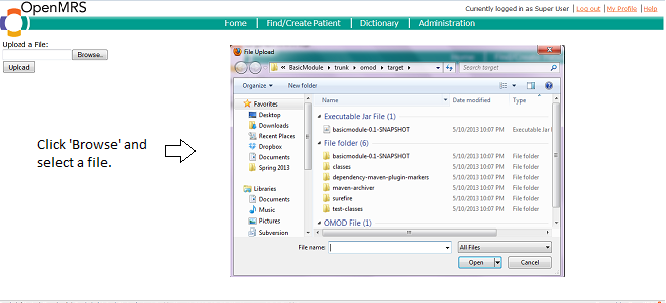
\includegraphics[width=6.5in]{user_guide/upload_browse.png}
\end{center}
\caption{DSS rule upload}
\label{fig:UPLOAD_BROWSE}
\end{figure}

\begin{figure}\begin{center}
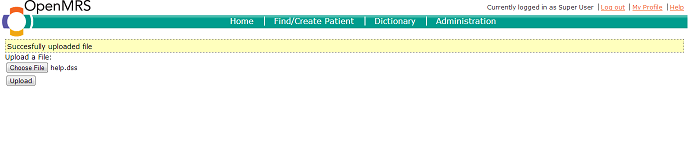
\includegraphics[width=6.5in]{user_guide/upload_success.png}
\end{center}
\caption{DSS rule upload confirmation}
\label{fig:UPLOAD_SUCCESS}
\end{figure}


\subsubsection{Load an existing rule}

Select an existing rule from the drop-down menu that you would like to modify then click 'Load'. (Figure ~\ref{fig:LOAD_RULE})
It will populate the textboxes under the “Create/Edit Rule” section. 
(Figure ~\ref{fig:LOAD_RULE_SHOWN})

Edit the file. Once complete, click 'Save'. A confirmation message will appear to ensure that you would like to overwrite an existing rule. Click yes to save the changes.
(Figure ~\ref{fig:MODIFY_CONFIRMATION})

A 'Successfully uploaded file' message will appear if there were no errors in the program. 
(Figure ~\ref{fig:MODIFY_ERROR})
If there are any errors, it will be reported back at the top of the page and it would not have saved the changes. 
(Figure ~\ref{fig:MODIFY_SUCCESS})
The code will still be available for you to work on it.

\begin{figure}\begin{center}
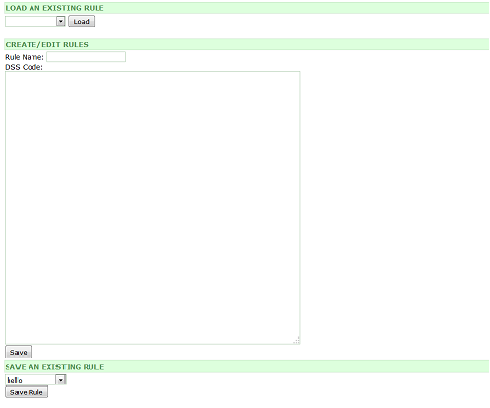
\includegraphics[width=6.5in]{user_guide/create_modify.png}
\end{center}
\caption{Create/Modify DSS Rule}
\label{fig:CREATE_MODIFY}
\end{figure}

\begin{figure}\begin{center}
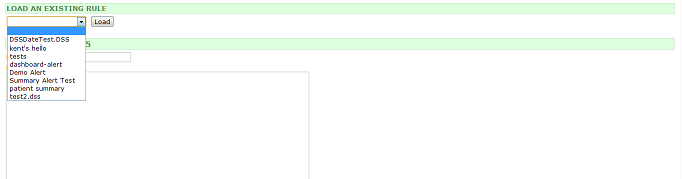
\includegraphics[width=6.5in]{user_guide/load_rule.png}
\end{center}
\caption{Loading an existing rule using the drop down menu}
\label{fig:LOAD_RULE}
\end{figure}

\begin{figure}\begin{center}
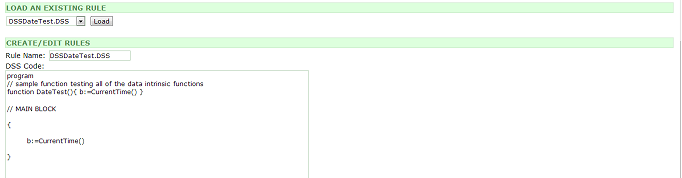
\includegraphics[width=6.5in]{user_guide/load_rule_shown.png}
\end{center}
\caption{Loaded rule displayed in text area}
\label{fig:LOAD_RULE_SHOWN}
\end{figure}

\begin{figure}\begin{center}
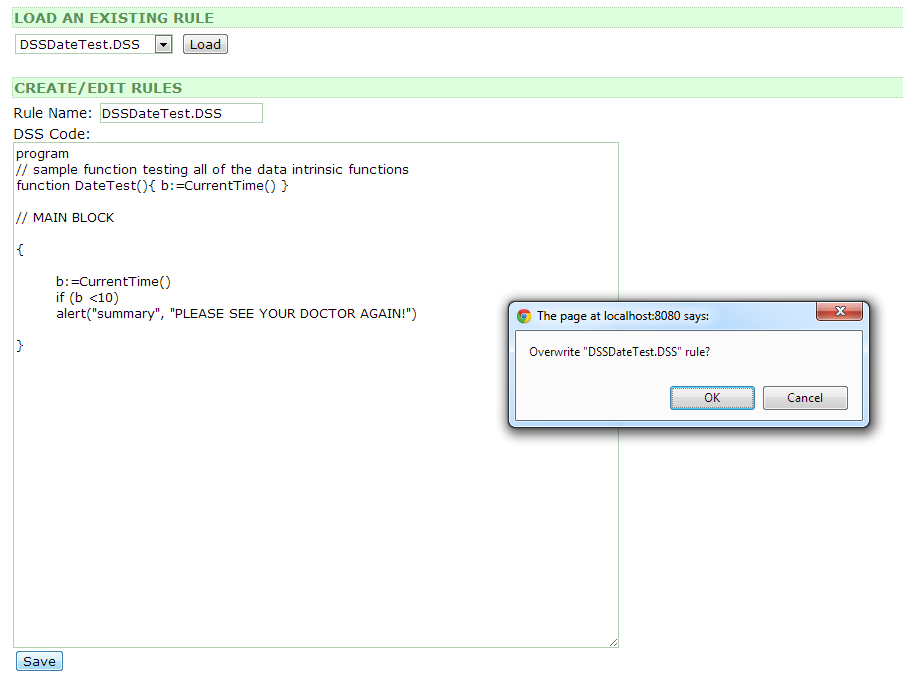
\includegraphics[width=6.5in]{user_guide/modify_confirmation.png}
\end{center}
\caption{Confirmation message, shown before over-writing an existing rule}
\label{fig:MODIFY_CONFIRMATION}
\end{figure}

\begin{figure}\begin{center}
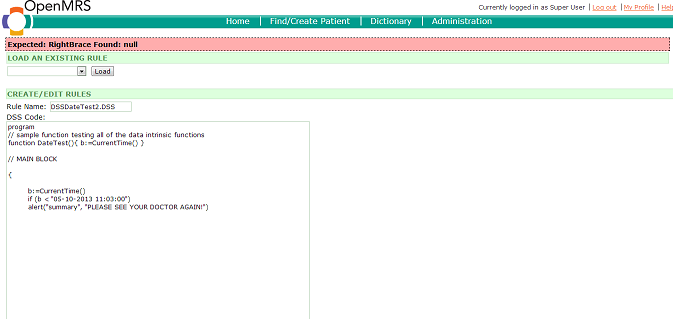
\includegraphics[width=6.5in]{user_guide/modify_error.png}
\end{center}
\caption{Error message shown when DSS code cannot be compiled}
\label{fig:MODIFY_ERROR}
\end{figure}

\begin{figure}\begin{center}
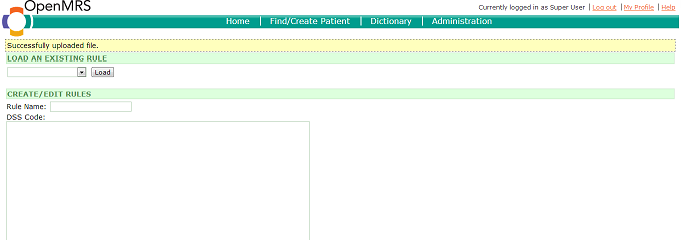
\includegraphics[width=6.5in]{user_guide/modify_success.png}
\end{center}
\caption{Confirmation message shown when DSS code has compiled successfully}
\label{fig:MODIFY_SUCCESS}
\end{figure}

\subsubsection{Create a rule}
You can create your own rule, it should not match an existing rule. Enter a rule name for the rule and enter the program under the textbox 'DSS Code' Once finished, click 'Save'.(Figure ~\ref{fig:NEW_RULE})

A 'Successfully uploaded file' message will appear if there were no errors in the program and the rule name will become available in the drop down menu. 
(Figure ~\ref{fig:NEW_RULE_SUCCESS})
If there are any errors, it will be reported back at the top of the page and it would not have saved the changes. The code will still be available for you to work on it.

\begin{figure}\begin{center}
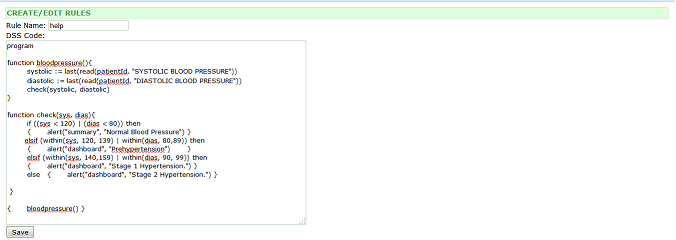
\includegraphics[width=6.5in]{user_guide/new_rule.png}
\end{center}
\caption{Creating a new rule}
\label{fig:NEW_RULE}
\end{figure}

\begin{figure}\begin{center}
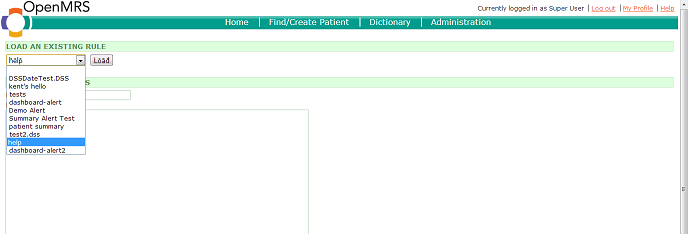
\includegraphics[width=6.5in]{user_guide/new_rule_success.png}
\end{center}
\caption{New rule after submission, shown in drop down menu}
\label{fig:NEW_RULE_SUCCESS}
\end{figure}

\subsubsection{Save an existing rule}
An existing rule can be saved on to your local file system. Choose the rule that you would like to save from the drop-down menu.
(Figure ~\ref{fig:SAVE_RULE})
Click 'Save Rule' and a download attachment window should appear. You can choose to either open the file or save the file. The file will be saved to your designated Downloads folder.
(Figure ~\ref{fig:SAVE_RULE_DIALOG})

\begin{figure}\begin{center}
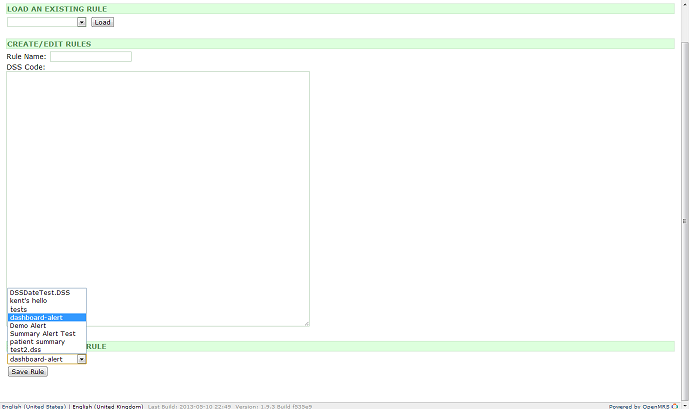
\includegraphics[width=6.5in]{user_guide/save_rule.png}
\end{center}
\caption{Choosing a rule to save locally}
\label{fig:SAVE_RULE}
\end{figure}

\begin{figure}\begin{center}
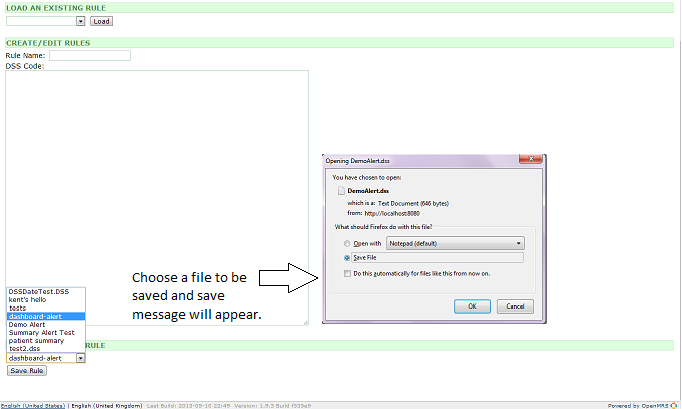
\includegraphics[width=6.5in]{user_guide/save_rule_dialog.png}
\end{center}
\caption{Browser dialog shown when attempting to save rule}
\label{fig:SAVE_RULE_DIALOG}
\end{figure}

\newpage 
\section{Use cases} \label{sec:USE_CASES}

Two main actors may interact directly with behaviors exposed in the 
DSS rule module: Administrators, who are responsible for maintaining 
the OpenMRS instance, and physicians, who utilize OpenMRS to 
support their interactions with patients. Either administrators 
or physicians may be responsible for authoring and maintaining 
rules, effectively creating a third category of actors. This 
distinction is relevant to understanding that physicians who see 
and respond to the alerts produced by rules may or may not be the 
same individuals who author those rules. Figure ~\ref{fig:USE_CASE_OVERVIEW} summarizes these interactions.

As a precondition to all use cases, an administrator is assumed to 
have installed the DSS rule module.

\begin{figure}\begin{center}
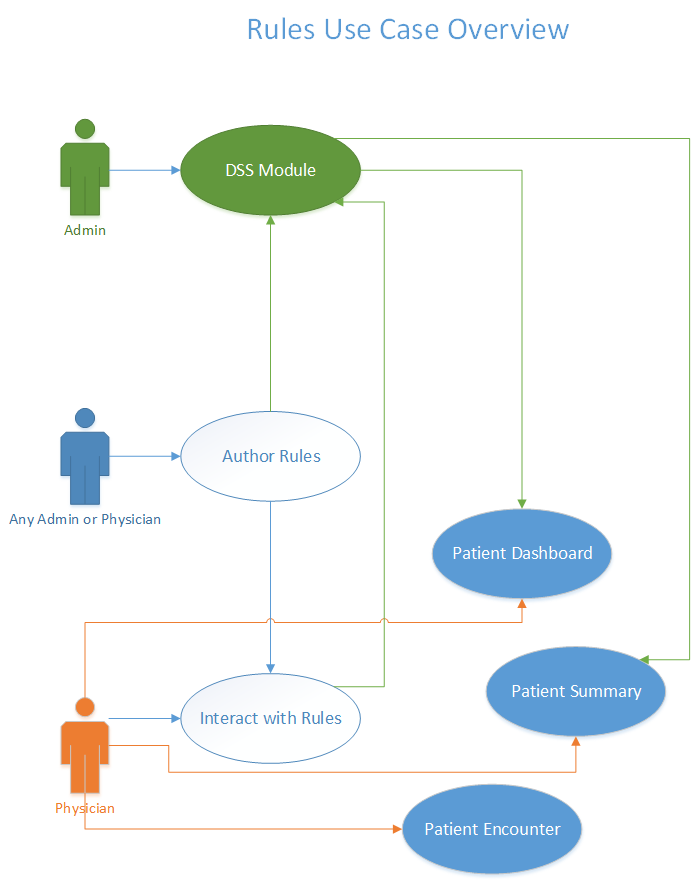
\includegraphics[height=6.5in]{use_case_overview.png}
\end{center}
\caption{Use case overview}
\label{fig:USE_CASE_OVERVIEW}
\end{figure}

\subsection{Authoring rules}

As discussed, a rule author may be either a physician or some 
form of administrator. Rule authorship and maintenance can be 
summarized by two tasks: Creating rules, described in 
Table ~\ref{tab:CREATE_RULE_USE_CASE} and 
Figure ~\ref{fig:CREATE_RULE_SEQUENCE},
and modifying existing rules, described in 
Table ~\ref{tab:MODIFY_RULE_USE_CASE} and 
Figure ~\ref{fig:MODIFY_RULE_SEQUENCE}.

\begin{table}
\begin{centering}
\begin{tabular}{ |  >{\bfseries}l | p{5in} |} \hline
Use case         &
1                \\ \hline
Use case name    &
Create Rule      \\ \hline
Summary          &
Administrator or physician can create, load, or edit rules. \\ \hline
Dependency       &
Knowledge of source code \\ \hline
Actor            &
Any administrator or physician \\ \hline
Precondition     &
Default settings \\ \hline
Description      &
Rule author navigates to Create/Modify DSS Rule page. \newline
Rule author enters a rule name and DSS Code. \newline
Rule is saved.    \newline
Rule author is able to edit or modify that rule. \\ \hline
Alternative      & 
If errors are present, rule author is notified. Rule entry form is 
not cleared, allowing error to be corrected.
\\ \hline
Postcondition    &
Rule is subsequently executed when navigating to patient 
summary or patient dashboard. \newline
Alerts produced by rule are shown where appropriate. \\ \hline
\end{tabular}
\end{centering}
\caption{Rule creation use case} \label{tab:CREATE_RULE_USE_CASE}
\end{table}

\begin{figure}\begin{center}
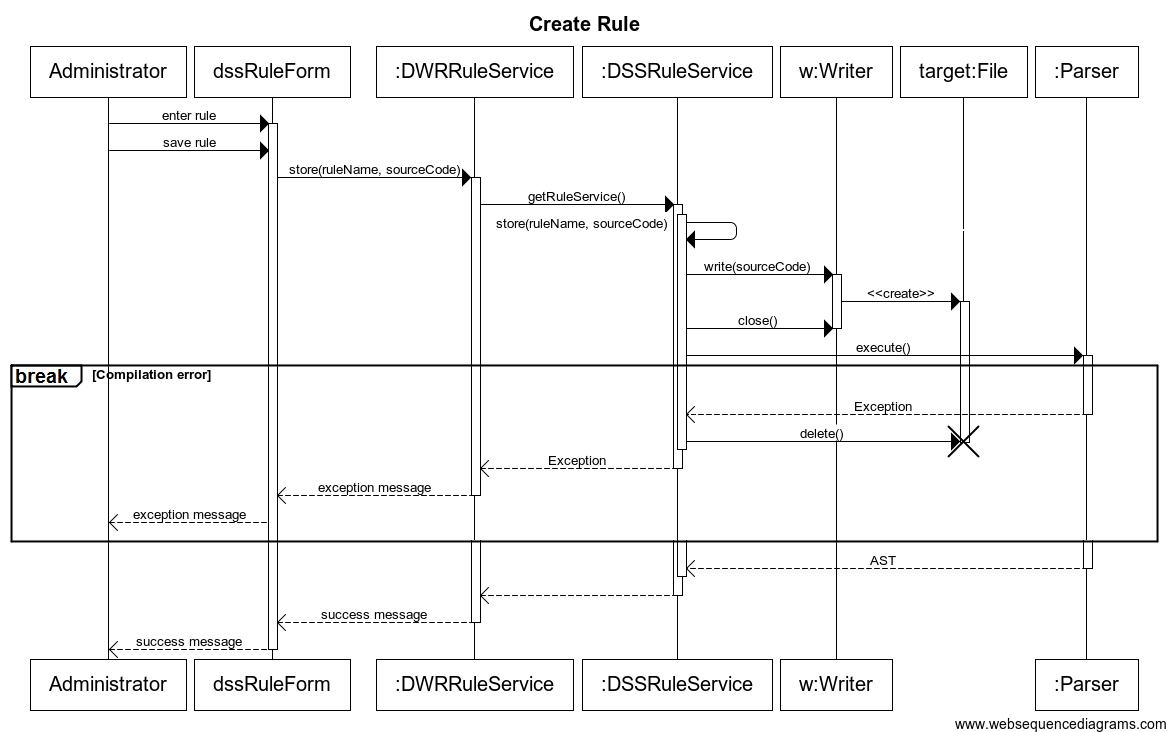
\includegraphics[width=6.5in]{sequence/create_rule.png}
\end{center}
\caption{Rule creation sequence diagram} 
\label{fig:CREATE_RULE_SEQUENCE}
\end{figure}


\begin{table}
\begin{centering}
\begin{tabular}{ |  >{\bfseries}l | p{5in} |} \hline
Use case &
2 \\ \hline
Use case name &
Modify Rule \\ \hline
Summary &
Administrator or physician can make changes to a rule. \\ \hline
Dependency &
Knowledge of source code \\ \hline
Actor &
Any adminstrator or physician \\ \hline
Precondition &
An existing rule previously saved \\ \hline
Description &
Rule author navigates to Create/Modify DSS Rule page. \newline
Rule author selects name of rule from drop down and hits "Load." \newline
Rule author makes necessary changes to a rule within the source code. \newline
Rule author hits save and confirms the modification when prompted.
\\ \hline
Alternative      & 
If errors are present, rule author is notified. Rule entry form is 
not cleared, allowing error to be corrected. \\ \hline
Postcondition &
Subsequent rule executions and alerts will exhibit the behavior specified in 
the modified rule.
 \\ \hline
\end{tabular}
\end{centering}
\caption{Rule modification use case} \label{tab:MODIFY_RULE_USE_CASE}
\end{table}

\begin{figure}\begin{center}
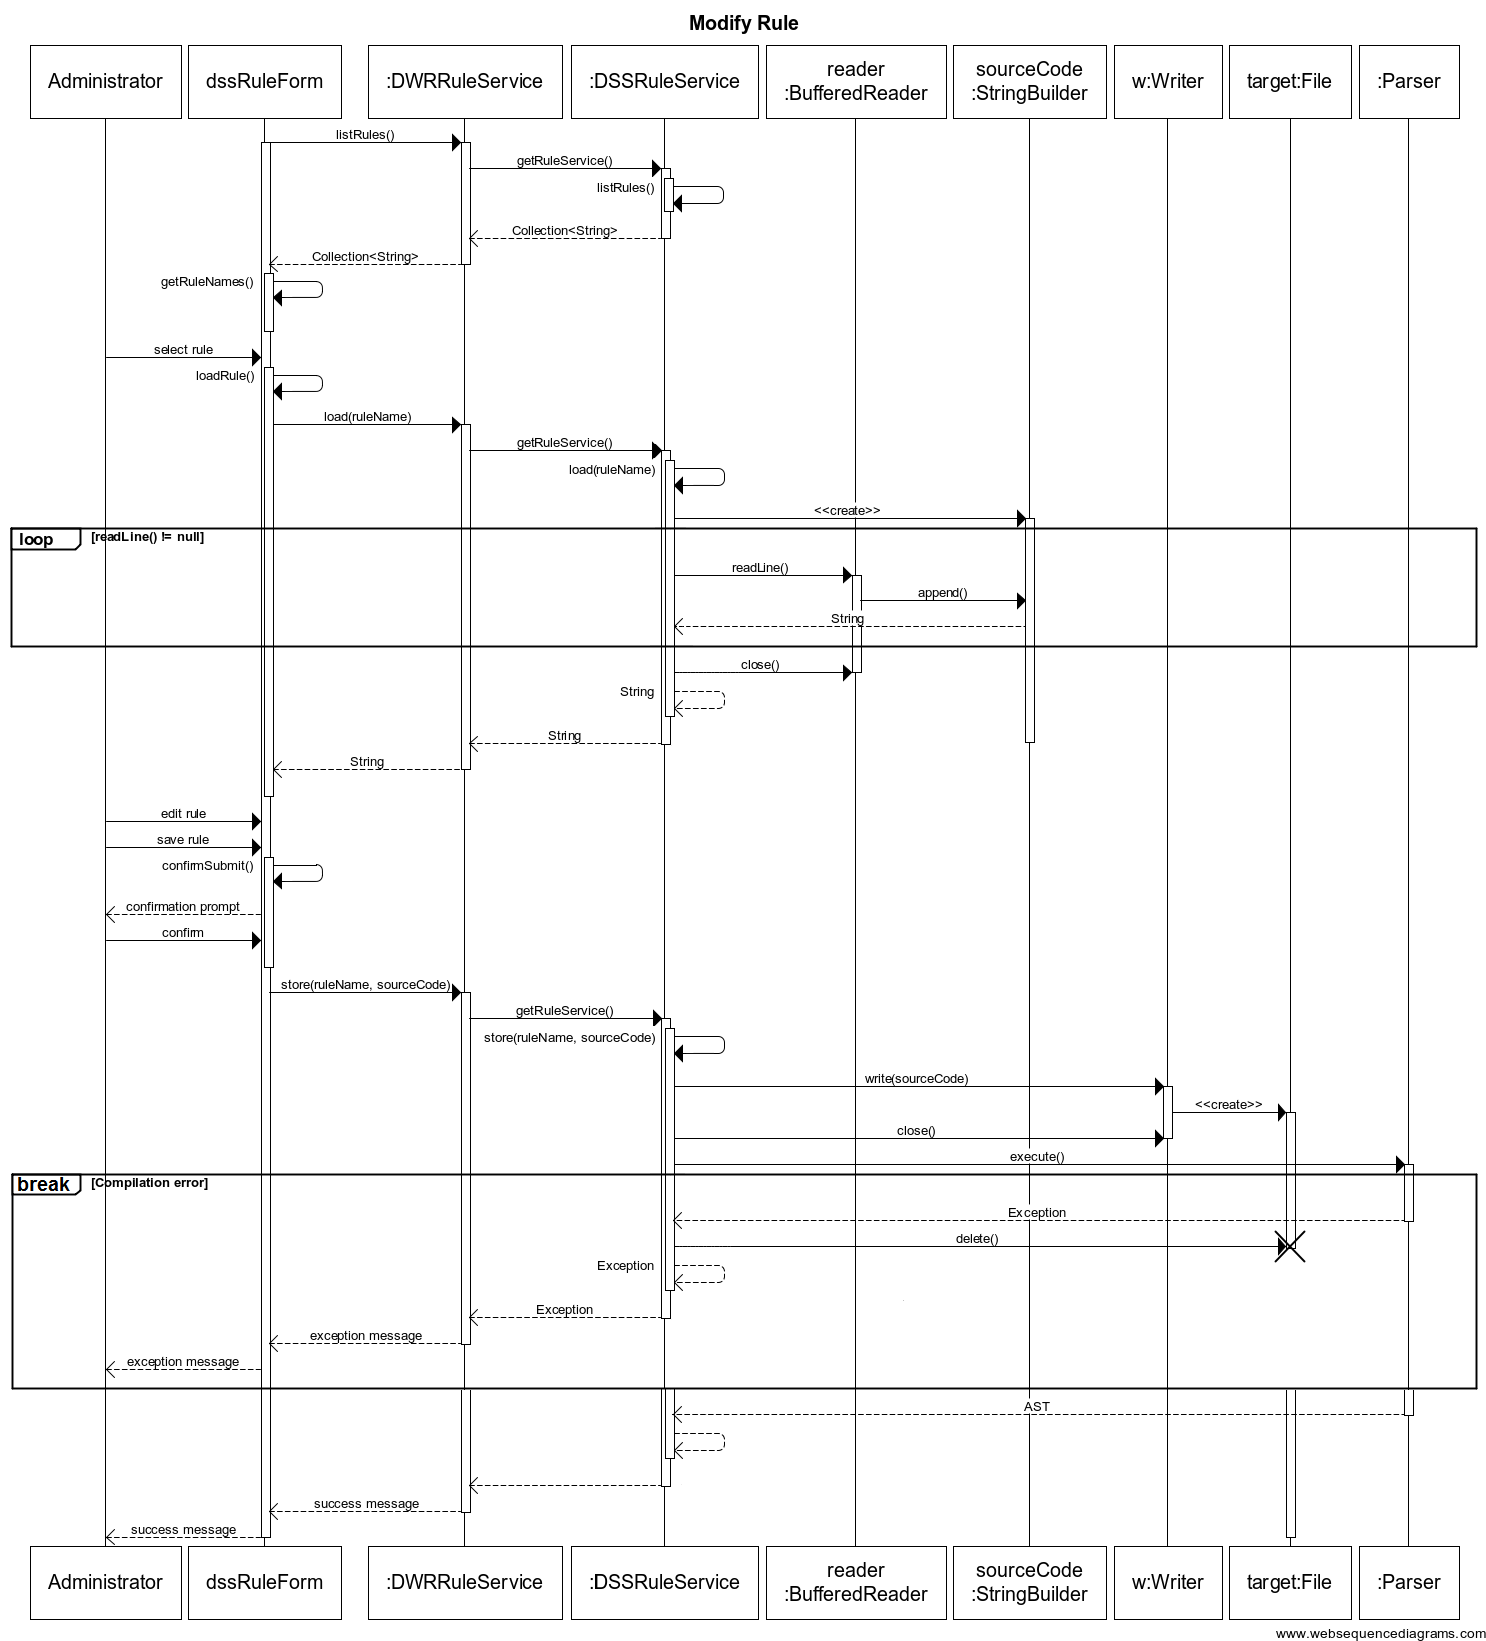
\includegraphics[width=6.5in]{sequence/modify_rule.png}
\end{center}
\caption{Rule modification sequence diagram} 
\label{fig:MODIFY_RULE_SEQUENCE}
\end{figure}

\subsection{Alerts}

The useful product of DSS rules is the alerts which they may generate, 
which can inform the actions a physician may subsequently take. Alerts 
are shown in two contexts: On the patient dashboard, as described in 
Table ~\ref{tab:PATIENT_DASHBOARD_USE_CASE} and 
Figure ~\ref{fig:PATIENT_DASHBOARD_SEQUENCE},
and within the patient summary, as described in 
Table ~\ref{tab:PATIENT_SUMMARY_USE_CASE} and 
Figure ~\ref{fig:PATIENT_SUMMARY_SEQUENCE}.

\begin{table}
\begin{centering}
\begin{tabular}{ |  >{\bfseries}l | p{5in} |} \hline
Use case &
3 \\ \hline
Use case name &
Patient Dashboard \\ \hline
Summary & 
Encounter information and relevant alerts are made available 
for a specific patient. \\ \hline
Dependency &
Log in to OpenMRS. \\ \hline
Actor &
Physician \\ \hline
Precondition &
An existing patient has been created. \\ \hline
Description &
Physician searches for a patient and navigates to patient dashboard. \newline
Medical information recorded on the patient is accessible through tabs for greater detail. \newline
Rules for patient are executed and any alerts for the "dashboard" target 
are displayed near the top of the page. \newline
A link to the Patient Summary page is provided near the top of the page.
\\ \hline
Alternative &
\\ \hline
Postcondition &
Physician may navigate among patient dashboard tabs containing 
patient information. \newline
Physician may navigate to patient summary. \newline
Physician has been notified with relevant alerts produced by defined 
DSS rules.
\\ \hline
\end{tabular}
\end{centering}
\caption{Patient dashboard use case} \label{tab:PATIENT_DASHBOARD_USE_CASE}
\end{table}

\begin{figure}\begin{center}
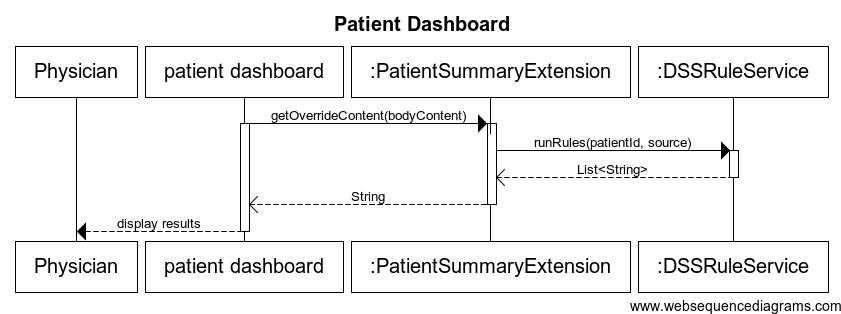
\includegraphics[width=6.5in]{sequence/patient_dashboard.png}
\end{center}
\caption{Patient dashboard sequence diagram} 
\label{fig:PATIENT_DASHBOARD_SEQUENCE}
\end{figure}

\begin{table}
\begin{centering}
\begin{tabular}{ |  >{\bfseries}l | p{5in} |} \hline
Use case &
4 \\ \hline
Use case name &
Patient Summary \\ \hline
Summary & 
Major information of a patient is displayed. \\ \hline
Dependency &
Patient Dashboard \\ \hline
Actor &
Physician \\ \hline
Precondition &
Relevant encounter data for the patient. \\ \hline
Description &
Physician clicks "Patient Summary" link from Patient Dashboard. \newline
Patient summary displays the main medical information including the WHO stage, TB Status, Allergies, and current drugs. \newline
Rules are executed, and any alerts for the "summary" target are 
displayed at the bottom of the page.
\\ \hline
Alternative &
\\ \hline
Postcondition &
Physician has summary information about the patient. \newline
Physician has been notified with relevant alerts produced by defined 
DSS rules.
\\ \hline
\end{tabular}
\end{centering}
\caption{Patient summary use case} \label{tab:PATIENT_SUMMARY_USE_CASE}
\end{table}

\begin{sidewaysfigure}\begin{center}
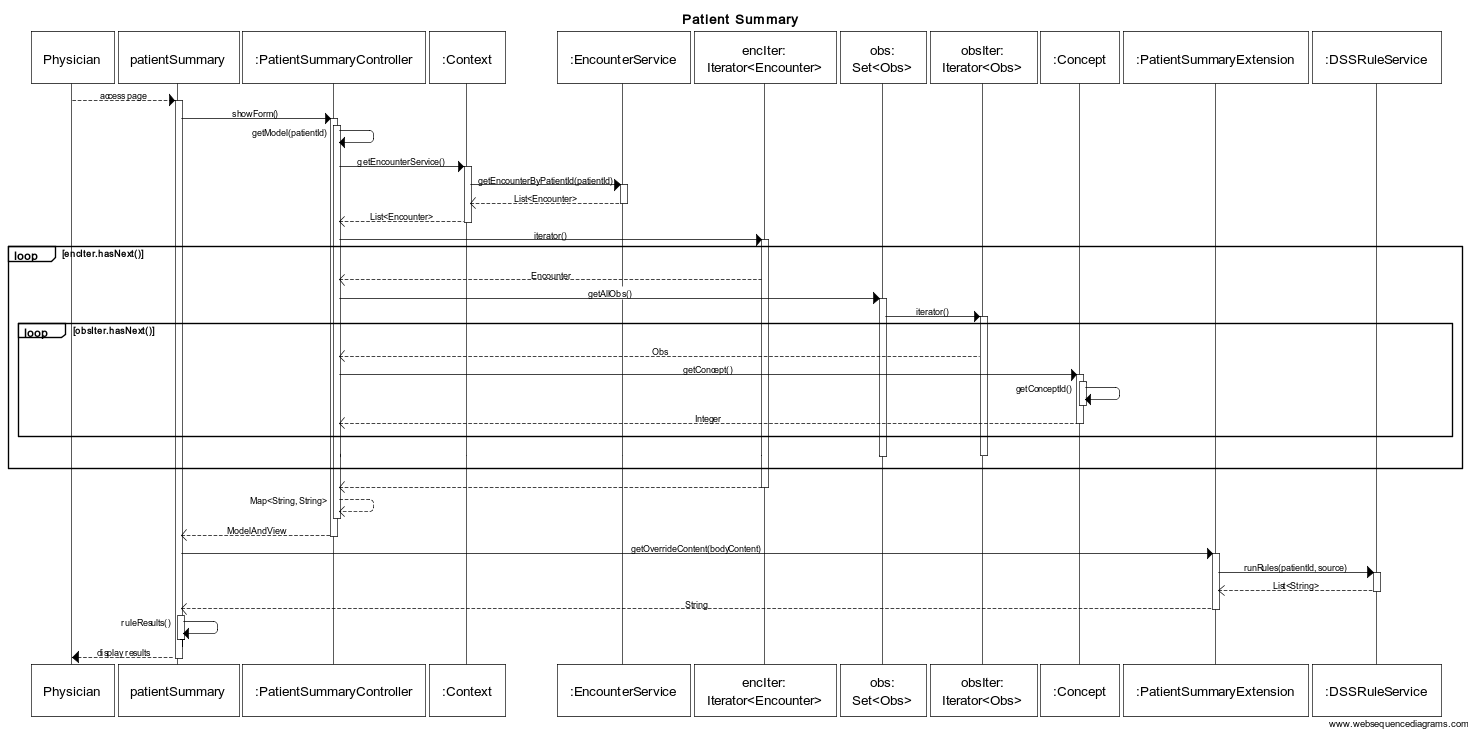
\includegraphics[width=8in]{sequence/patient_summary.png}
\end{center}
\caption{Patient summary sequence diagram} 
\label{fig:PATIENT_SUMMARY_SEQUENCE}
\end{sidewaysfigure}


\newpage 
\section{Design overview} \label{sec:DESIGN_OVERVIEW}

	The DSS1 rule subsystem is incorporated into OpenMRS in a simple Client-Server fashion. The target implementation will feature client-side web pages which interact with the DSS1 rule subsystem on the server by way of DSSRuleService. Figure ~\ref{fig:TIERS} illustrates this interaction.

\tikzstyle{layer}=[rectangle, 
                   rounded corners,
                   draw=black, 
                   align=center,
                   anchor=north]
\tikzstyle{communicates}=[draw, ->, >=triangle 60]
\tikzstyle{boundary}=[draw, -, dashed]
\begin{figure}\begin{center}
\begin{tikzpicture}
\node (Client) [layer] { 
  \textbf{Client Pages}      \\
  Patient Summary \\
  Patient Dashboard \\
  DSS Rule Administration
};
\node (Boundary) [below=of Client, minimum width=3in] {};
\node [above=of Boundary.east] {\emph{Client}};
\node [below=of Boundary.east] {\emph{Server}};
\node (Service) [layer, below=of Boundary] { 
  \textbf{DSS Rule Service}  \\
  Run rules  \\
  List rules \\
  Add rules  \\
  Edit rules
};
\node (Interpreter) [layer, below=of Service] { 
  \textbf{DSS1 Interpreter}  \\
  Intrinsics  \\
  Evaluations \\
  Flow control
};
\path [communicates] (Client) -- (Service) {};
%\path [communicates] (Service.115    ) -- (Client.240     ) {};
\path [communicates] (Service) -- (Interpreter) {};
%\path [communicates] (Interpreter.120) -- (Service.245    ) {};
\path [boundary] (Boundary.180) -- (Boundary.0    ) {};
%\path [boundary]     (Boundary.west  ) -- (Boundary.east  ) {};
\end{tikzpicture}
\caption{Usage relationship of major tiers.}\label{fig:TIERS}
\end{center}\end{figure}

The DSS Rule Service, in turn, utilizing the DSS1 Interpreter subsystem to run rules and report results.

While the DSS Rule Service runs on the server, its interface is exposed to client-side JavaScript code via DWR (Direct Web Remoting).

\subsection{Client pages} \label{sec:CLIENT_PAGES}

Multiple client web pages interact with the DSS Rule Service.

\subsubsection{Patient summary} \label{sec:PATIENT_SUMMARY}

The Patient Summary ({\texttt{patientsummary.jsp}) is  stand-alone page, reachable from a link on the Patient Dashboard. It is used primarily to contain major information about a patient (gender, age, WHO stage, etc.) The Patient Summary invokes the rule service via DWR to retrieve all alerts for the named target  \texttt{summary} and displays them below other patient information. 

\subsubsection{Patient Dashboard} \label{sec:PATIENT_DASHBOARD}

The Patient Dashboard is the primary landing point for viewing patient information, and contains multiple tabs for this purpose. This extension inserts a link to the Patient Summary on the Patient Dashboard, and accompanies this with relevant alerts by invoking the rule service for the \texttt{dashboard} target.

See \texttt{org.openmrs.module.basicmodule.extension.html.PatientSummaryExtension}

\subsubsection {DSS Rule Administration} 
\label{sec:DSS_RULE_ADMINISTRATION}

Create DSS Rule (\texttt{dssRules.form}) provides a form where DSS source code can be entered and submitted to the rule service with a specific rule name. Consolidates the ability to create new rules, load existing rules, and edit rules in one form. Made accessible through an extension to the Administration menu.

\subsection{Rule service} \label{sec:RULE_SERVICE}

The DSSRuleService follows the facade design pattern to expose important functionality to clients. The high-level tasks that are relevant to client code are defined using a few simple methods which hide the details of compiling, interpreting, and managing the storage of rules. Specific functionality is detailed in table ~\ref{tab:RULE_SERVICE}.

\begin{table}
\begin{center}
\begin{tabular}{ l | p{1.25in} | p{2.25in} }
Method & Description & Details \\ \hline

\texttt{getRuleService()}
&
Static method to retrieve an instance of the rule service.
&
Constructs a new DSSRuleService object, if necessary. During 
constructor call any existing rules are loaded from the file 
system, using the XMLBuilder to convert from XML to DOM to AST.
\\ \hline

\texttt{store(rule, code)}
&
Stores a rule (either as a new rule, or replacing an existing rule) with the given source code.
&
Invokes the Parser to convert source code to AST; 
Invokes the XMLBuilder to convert AST to DOM and save; 
Saves the original source to file system for subsequent retrieval; 
Stores the AST in memory for subsequent running.
\\ \hline

\texttt{load(rule)}
&
Load the source code for an existing rule.
&
Reads stored source code from the file system.
\\ \hline

\texttt{listRules()}
&
List all existing rules.
&
Returns a list of all stored rule names.
\\ \hline

\texttt{runRules(patientId, target)}
&
Get all alerts for the given target (“summary” or “dashboard”) as appropriate to the given patient.
&
For each rule:
Construct interpreter; 
Install intrinsics, including “alert” function which stores to a map;
Pre-define “patientId” for DSS1 program;
Run the interpreter on the rule.
Thereafter, pull all alerts appropriate to the target from the map.
\\ \hline

\end{tabular}
\end{center}
\caption{Methods exposed by the DSS Rule Service}
\label{tab:RULE_SERVICE}
\end{table}

\subsubsection{Rule storage} \label{sec:RULE_STORAGE}

On upload, rules are compiled to an Abstract Syntax Tree (AST) form 
using the provided Parser class. Once compiled successfully, the rule is stored to the OpenMRS application data directory. 

Each rule is  stored in two formats: Plain text source code, and an XML (Extensible Markup Language) representation of the compiled AST. The 
source code is subsequently used only to support user interactions (for instance, if an administrator wants to load or modify source for an existing rule). The XML form is used when the DSS Rule Service is first initialized to load any existing rules from the file system. After initialization, rules are stored in memory as AST objects.

The utility class XMLBuilder is used for conversion between AST and XML. Internally, the class maintains a Document Object Model (DOM) representation of the AST. This can be either as loaded from an XML file, or as formed by traversing an AST. Likewise, XMLBuilder provides methods for both producing AST objects or writing XML files.

\subsection{Interpreter} \label{sec:INTERPRETER}

The Interpreter is implemented with four distinct sub systems, as depicted in Figure ~\ref{fig:INTERPRETER}.
At the top level, \emph{flow control} is provided by the InterpreterVisitor, which is responsible for traversing the Abstract Syntax Tree. An \emph{execution context} is maintained to describe the running state of the system, including defined variables and functions. While tree traversal coordinates complex expressions, the actual \emph{evaluation} of expressions is itself implemented in a distinct set of classes representing the types available under DSS1. Finally, a library of \emph{intrinsic functions} is provided in order to mediate interactions with OpenMRS from running DSS1, as well as to provide certain convenience functions to DSS1 rule programmers.

\tikzstyle{system}=[rectangle,
                   thick, 
                   draw=black, 
                   align=center,
                   anchor=north]
\tikzstyle{connects}=[draw, ->, >=triangle 60]
\tikzstyle{observes}=[draw, ->, dashed, >=triangle 60]
\begin{figure}
\begin{center}
\begin{tikzpicture}[node distance=1.5in]
\node (FlowControl) [system] 
      {\textbf{Flow control}};
\node (Middle) [below=of FlowControl] {};
\node (ExecutionContext) [system, left=of Middle] 
      {\textbf{Execution context}};
\node (Evaluation) [system, below=of Middle] 
      {\textbf{Evaluation}};
\node (IntrinsicFunction) [system, right=of Middle] 
      {\textbf{Intrinsic functions}};
\draw [connects] (FlowControl) -- (ExecutionContext) {}
      node [midway,above,sloped] {Sets, gets state} ;
\draw [connects] (ExecutionContext) -- (Evaluation) {}
      node [midway,below,sloped] {Contains values} ;
\draw [connects] (ExecutionContext) -- (IntrinsicFunction) {}
      node [midway,below left,sloped] {Contains functions} ;
\draw [connects] (FlowControl) -- (IntrinsicFunction) {}
      node [midway,above,sloped] {Invokes} ;
\draw [connects] (IntrinsicFunction) -- (Evaluation) {}
      node [midway,below,sloped] {Yields values} ;
\draw [connects] (FlowControl) -- (Evaluation) {}
      node [midway,above,sloped] {Assembles complex expressions} ;
\end{tikzpicture}
\end{center}
\caption{High-level overview of the DSS1 Interpreter.}
\label{fig:INTERPRETER}
\end{figure}

\subsubsection{Flow control} \label{sec:FLOW_CONTROL}

	Flow control in the interpreter is implemented using the Visitor design pattern, traversing the Abstract Syntax Tree (AST) produced by the existing Compiler using an implementation of the provided ASTVisitor interface, performing computation as appropriate at every given node in the tree.

	The Visitor design pattern leverages double dispatch to decouple a data structure from the operations which can be performed while traversing this data structure. The Visitor calls an \texttt{accept} method on a node within the data structure, which is itself overloaded to call a more specific method on the Visitor itself; \texttt{visitBlockTree}, for example. This permits the external object – the Visitor – to implement behavior using the data structure's type hierarchy, without adding that specific behavior to those types directly.

	In the case of the Interpreter, the data structure is the AST, which describes a DSS1 program as a tree of elements – block (BlockTree), if statements (IfTree), et cetera. The Visitor is the IntepreterVisitor, which manages and performs the computation described by this program. This is done with the support of other underlying subsystems to describe variable state and perform type-specific evaluations, as described in the Architecture section.

	The class InterpreterVisitor acts as the center of a subsystem  responsible for high-level interpretation of the program, including flow control, and coordinating complex expressions.

\subsubsection{Execution context} \label{sec:EXECUTION_CONTEXT}

The ExecutionContext class provides a means to store and retrieve return values, variable states, and named functions. It also handles rules of scope to hide variables during function calls, and exposes the Evaluator. Note that this may be populated with functions or even variables before being given to the InterpreterVisitor, allowing the definition of intrinsics and constants (such as \texttt{patientId}).

Functions stored in the ExecutionContext are of type DSSFunction, which is an interface used to describe any function called from DSS1 (either intrinsic or user-defined). This permits function calling to be implemented identically for both categories of function. Additionally includes a method for testing if a given argument should be passed as a raw identifier instead of evaluated directly (as used by some intrinsics.).

Similarly, variables and return values are stored as DSSValue 
objects, with their specific implementation defined within the 
evaluation subsystem.

\subsubsection{Evaluation of expressions} \label{sec:EVALUATION}

The abstract class DSSValue describes a set of operations which can be performed on values in DSS1 as methods, as well as the common state (the potential to store time stamps). Its concrete sub-classes, such as DSSValueInt, DSSValueFloat, et cetera, provide specific implementations of these operations in order to define the behavior of their DSS1 type. Additionally, concrete subclasses of DSSValue typically are defined with some field to maintain their specific value (for instance, DSSValueBool has an underlying Java \texttt{boolean} field to describe its value.)

The Evaluator interface and DSSEvaluator implementation exposes methods to perform operations upon DSS1 values, to interpret literals, allocate DSS objects, and perform conversions between DSS1 values and similar Java objects. The Evaluator serves as intermediary between flow control and the specific semantics implemented in DSSValue types; this facilitates separation of concerns, allowing the gradual introduction of new DSS1 data types while avoiding changes to  flow control.

Finally, a DSSValueFactory class is provided to aid in the instantiation of DSSValue objects. This class utilizes the Factory design pattern to allow new values to be created (for instance, as the return values of intrinsic functions) without requiring users of those values to have specific knowledge of the DSSValue subclasses actually used.

\subsubsection{Intrinsic functions} \label{sec:INTRINSIC_FUNCTIONS}

DSSLibrary defines an interface for delivering or generating intrinsic functions in related groupings. Each function is returned in a map where the name should be used to call the function from a DSS program, and the function object is used as a Java object that extends the DSSFunction. These functions may then be easily installed into the ExecutionContext used by the Intepreter before running rules. A list of libraries used in this implementation is presented in Table ~\ref{tab:LIBRARIES}.

This approach supports extensibility of the DSS rule module. 
Rather than being built into the DSS1 Interpreter at the language 
level, intrinsic functions can be contained and communicated 
as DSSLibrary objects. Adding intrinsics is then as simple as 
defining a new DSSLibrary and installing it to the execution context before running rules.

The ReadLibrary serves as an interesting example case, at it illustrates interaction with the OpenMRS platform without requiring specific knowledge of this platform from other elements of the interpreter. The read functions retrieve a list of observations associated with a patient. The first parameter of the functions, patientId, is a numeric identifier unique to each patient. The second parameter, conceptName, is the word or phrase used by the OpenMRS dictionary to refer to a concept. 

The three functions are nearly identical, save for one difference: while read() returns a list containing all observations that match the function parameters, readInitialEncounter() and readLatestEncounter() filter out results based on the timestamp of the observations. Calling readInitialEncounter() retrieves only the observations from the patient's earliest encounter on record, while readLatestEncounter() retrieves only the observations from the patient's most recent encounter on record. 

When the functions are called, they retrieve a list of all encounters associated with patientId from the OpenMRS database. The functions iterate through these lists, and in the case of readInitialEncounter() and readLatestEncounter(), the timestamp for each encounter is checked. If the timestamp does not meet the criteria, the encounter is discarded. Once an encounter has been verified as valid the function shall retrieve all observations associated with the encounter. Each observation shall have its concept name checked against conceptName, and matches are added to the list of observations that each function shall return. 

Observations consist of three pieces of data: the value of the observation, the data type of the observation value, and the time of the observation. Internally, observations are represented as DSSValue objects, which store the value of the observation and the time of the observation. The data type of the observation value is stored as part of the DSSValue class type itself. Both the time and data type of the observation can be retrieved using the time() and type check intrinsics, respectively. 

Note that the \texttt{alert} intrinsic is treated as a special case. Rather than being contained within a library class, it is installed directly by the DSS Rule Service into the Interpreter before running rules. This facilitates retrieval of results issued via \texttt{alert} calls.

\begin{table}
\begin{center}
\begin{tabular} { l | l }
\textbf{Library}  & \textbf{Functions implemented}\\ \hline
IsLibrary         & \texttt{isString(var)}        \\
                  & \texttt{isFloat(var)}         \\
                  & \texttt{isInt(var)}           \\
                  & \texttt{isBoolean(var)}       \\
                  & \texttt{isList(var)}          \\
                  & \texttt{isObject(var)}        \\
                  & \texttt{isDate(var)}          \\ \hline
LengthAndWithinLibrary
                  & \texttt{length(var)}          \\
                  & \texttt{within(v,a,b)}        \\ \hline
ListLibrary       & \texttt{merge(a,b)}           \\
                  & \texttt{sortTime(list)}       \\
                  & \texttt{sortData(list)}       \\
                  & \texttt{first(list)}          \\
                  & \texttt{last(list)}           \\ \hline
ReadLibrary       & \texttt{read(patientId,
                                 concept)}        \\
                  & \texttt{readInitialEncounter(patientId,
                                 concept)}        \\
                  & \texttt{readLatestEncounter(patientId,
                                 concept)}        \\ \hline
DateLibrary       & \texttt{currenttime()}        \\
                  & \texttt{recentTimeItem(list)} \\
                  & \texttt{oldestTimeItem(list)} \\
                  & \texttt{before(a,b)}          \\
                  & \texttt{time(var)}            \\
                  & \texttt{addDays(v,days)}      \\
                  & \texttt{addMonths(v,months)}  \\ \hline
\end{tabular}
\end{center}
\caption{Libraries of intrinsics}
\label{tab:LIBRARIES}
\end{table}

% \section{External documentation}

\newpage 
\section{Package diagrams}

\newpage 
\section{Class diagrams} \label{sec:CLASS_DIAGRAMS}

\subsection{Classes describing flow control}

Figure ~\ref{fig:INTERPRETER_VISITOR_DIAGRAM} shows the relationship 
of classes directly involved in or utilized during the handling of flow 
control when interpreting a DSS program.

The InterpreterVisitor is used to initiate program interpretation. It 
delegates the interpretation of specific node types to corresponding 
ASTInterpreter types. It also maintains an instance of a DSSExecutionContext 
to support interactions with the running state of the program.

\subsection{Classes describing execution context}

Figure ~\ref{fig:EXECUTION_CONTEXT_DIAGRAM} describes the 
composition of the execution context. The active state of the program, 
including currently-defined functions and variable assignments, is maintained in appropriate data structures.

Each ExecutionContext additionally maintains a reference to an Evaluator 
object, which exposes necessary methods for the interpreter to interact 
with values in DSS.

\subsection{Classes describing values}

Figure ~\ref{fig:VALUE_DIAGRAM} shows the classes used to describe values in 
a running DSS program. The abstract class DSSValue describes the operations 
available under DSS1 as methods; its concrete subclasses provide 
implementations for these operations. Note that each DSSValue object also 
maintains a field for the time stamp of a value, which is populated when 
observations are read from OpenMRS services. For other values this is null.

Not shown is DSSValueFactory, which exposes methods to create DSSValue 
objects to wrap their corresponding underlying Java types.

\subsection{Classes describing intrinsics}

Figure ~\ref{fig:INTRINSIC_DIAGRAM} describes the relationship of classes 
which describe specific intrinsic functions to the classes used to 
categorize them.

Calls made by a running DSS program are resolved by a named DSSFunction 
object, as stored in the execution context. The DSSLibrary interface 
provides a useful way to group related functions along with their names 
to facilitate their installation into the execution context. 

Also shown is the DeclaredFunction class. A DeclaredFunction is created 
for user-defined functions in a DSS program, and contains references to 
appropriate nodes within the AST to support actual interpretation of the 
function call, as well as the visitor used to perform interpretation, and 
the execution context, which is used to handle the change in variable 
scope associated with the function call.

\tikzstyle{class}=[rectangle, 
                   draw=black, 
                   rectangle split, 
                   rectangle split parts=3,
                   align=center,
                   anchor=north]
\tikzstyle{implements}=[draw, ->, >=open triangle 90]
\tikzstyle{aggregates}=[draw, <-, >=open diamond]
\tikzstyle{contains}=[draw, <-, >=diamond]

\begin{figure}
\begin{center}
\begin{tikzpicture}[node distance=0.25in]
\node (ASTVisitor) [class] { 
  \emph{ASTVisitor}
  \nodepart{second}  
  \nodepart[align=justify]{third}
  + visitBlockTree(t : AST) \\
  + visitIdTree(t : AST)    \\
  + visitCallTree(t : AST)  \\
  ...
};
\node (InterpreterVisitor) [class, below=of ASTVisitor] { 
  \textbf{InterpreterVisitor}
  \nodepart{second}  
  \nodepart[align=justify]{third}
};

\node (DSSExecutionContext) [class, right=of InterpreterVisitor] { 
  \textbf{DSSExecutionContext}
  \nodepart{second}  
  \nodepart[align=justify]{third}
  + setConstant(name : String,  value : DSSValue) \\
  + setIntrinsic(name : String,  func : DSSFunction)
};
\node (ExecutionContext) [class, above=of DSSExecutionContext] { 
  \textbf{ExecutionContext}
  \nodepart[align=justify]{second}  
  - evaluator : Evaluator
  \nodepart[align=justify]{third}
  + beginScope() \\
  + endScope() \\
  + getEvaluator() : Evaluator \\
  + getFunction(name : String) : DSSFunction \\
  + getReturnValue() : DSSValue \\
  + setReturnValue(v : DSSValue) \\
  + setFunction(name : String, f : DSSFunction)
};
\node (ASTInterpreter) [class, below=of InterpreterVisitor.south east] { 
  \emph{ASTInterpreter}
  \nodepart{second}  
  \nodepart[align=justify]{third}
  + interpret(ast : AST, 
              c : ExecutionContext, 
              v : ASTVisitor) \\ \hspace{10pt} : Object
};

\node (IdInterpreter) [class, below=of ASTInterpreter] { 
  \textbf{IdInterpreter}
  \nodepart{second}  
  \nodepart[align=justify]{third}
};
\node (BlockInterpreter) [class, left=of IdInterpreter] { 
  \textbf{BlockInterpreter}
  \nodepart{second}  
  \nodepart[align=justify]{third}
};
\node (CallInterpreter) [class, right=of IdInterpreter] { 
  \textbf{CallInterpreter}
  \nodepart{second}  
  \nodepart[align=justify]{third}
};
\node () [right=of CallInterpreter] {...};


\node (NamingContext) [class, above=of ExecutionContext] { 
  \emph{NamingContext}
  \nodepart[align=justify]{third}
  +set (name : String, value : DSSValue) \\
  +get (name : String) : DSSValue
};

\path [implements] (ExecutionContext) -- (NamingContext) {};
\path [implements] (InterpreterVisitor) -- (ASTVisitor) {};
\path [implements] (BlockInterpreter) -- (ASTInterpreter) {};
\path [implements] (IdInterpreter) -- (ASTInterpreter) {};
\path [implements] (CallInterpreter) -- (ASTInterpreter) {};
\path [implements] (DSSExecutionContext) -- (ExecutionContext) {};
\path [contains] (InterpreterVisitor) -- (DSSExecutionContext) {};
\path [contains] (InterpreterVisitor) -- (ASTInterpreter) {};
\draw (InterpreterVisitor) -- (ASTInterpreter) 
      node [midway, right] {\small{1..*}};
\draw (InterpreterVisitor) -- (DSSExecutionContext) 
      node [midway, above] {\small{1..1}};
\end{tikzpicture}
\end{center}
\caption{Interpreter visitor}
\label{fig:INTERPRETER_VISITOR_DIAGRAM}
\end{figure}

\begin{figure}
\begin{tikzpicture}[node distance=0.33in]
\node (ExecutionContext) [class] { 
  \textbf{ExecutionContext}
  \nodepart[align=justify]{second}  
  - functions : Map\textless String, DSSFunction\textgreater \\
  - variables : Map\textless String, DSSValue\textgreater \\
  - scope : Stack\textless Map\textless String, DSSValue\textgreater \textgreater \\
  - returnValue : DSSValue \\
  - evaluator : Evaluator
  \nodepart[align=justify]{third}
  + beginScope() \\
  + endScope() \\
  + getEvaluator() : Evaluator \\
  + getFunction(name : String) : DSSFunction \\
  + getReturnValue() : DSSValue \\
  + setReturnValue(v : DSSValue) \\
  + setFunction(name : String, f : DSSFunction)
};
\node (DSSValue) [class, right=of ExecutionContext] { 
  \emph{DSSValue}
  \nodepart[align=justify]{second}  
  - timestamp : Date
  \nodepart[align=justify]{third}
  + add (v : DSSValue) : DSSValue \\
  + sub (v : DSSValue) : DSSValue \\
  + div (v : DSSValue) : DSSValue \\
  ... \\
  + getTimeStamp() : Date
};
\node (NamingContext) [class, above=of ExecutionContext] { 
  \emph{NamingContext}
  \nodepart[align=justify]{third}
  +set (name : String, value : DSSValue) \\
  +get (name : String) : DSSValue
};
\node (DSSFunction) [class, right=of NamingContext] { 
  \emph{DSSFunction}
  \nodepart{second}  
  \nodepart[align=justify]{third}
  + call(args : DSSValue[]) : DSSValue \\
  + passAsIdentifier(argIndex : int) \\ \hspace{10pt} : boolean
};

\node (Evaluator) [class, below=of ExecutionContext] { 
  \emph{Evaluator}
  \nodepart{second}  
  \nodepart[align=justify]{third}
  + castTo(javaClass : Class, v : DSSValue) : Object \\
  + evaluate(leftOper : DSSValue, \\ 
    \hspace{10pt} operator : String, \\
    \hspace{10pt} rightOper : DSSValue) : DSSValue\\
  + evaluateLiteral(lit : Symbol) : DSSValue \\
  + newAllocation(fields : String[]) : DSSValue \\
  + toDSSValue(javaObject : Object) : DSSValue
};
\node (DSSEvaluator) [class, right=of Evaluator] { 
  \textbf{DSSEvaluator}
  \nodepart{second}  
  \nodepart[align=justify]{third}
};


\path [aggregates] (ExecutionContext) -- (DSSValue) {};
\path [aggregates] (ExecutionContext) -- (DSSFunction) {};
\path [contains] (ExecutionContext) -- (Evaluator) {};
\path [implements] (ExecutionContext) -- (NamingContext) {};
\path [implements] (DSSEvaluator) -- (Evaluator) {};
\draw (ExecutionContext) -- (DSSValue) 
      node [midway, above] {\small{1..*}};
\draw (ExecutionContext) -- (DSSFunction) 
      node [midway, below] {\small{1..*}};

\end{tikzpicture}
\caption{Execution context class diagram}
\label{fig:EXECUTION_CONTEXT_DIAGRAM}
\end{figure}

\begin{figure}
\begin{center}
\begin{tikzpicture}[node distance=0.25in]
\node (DSSValue) [class] { 
  \emph{DSSValue}
  \nodepart[align=justify]{second}  
  - timestamp : Date
  \nodepart[align=justify]{third}
  + add (v : DSSValue) : DSSValue \\
  + sub (v : DSSValue) : DSSValue \\
  + div (v : DSSValue) : DSSValue \\
  + mul (v : DSSValue) : DSSValue \\
  + power (v : DSSValue) : DSSValue \\
  + concat (v : DSSValue) : DSSValue \\
  + and (v : DSSValue) : DSSValue \\
  + or (v : DSSValue) : DSSValue \\
  + equal (v : DSSValue) : boolean \\
  + notequal (v : DSSValue) : boolean \\
  + lessthan (v : DSSValue) : boolean \\
  + greaterthan (v : DSSValue) : boolean \\
  + lessthanequal (v : DSSValue) : boolean \\
  + greaterthanequal (v : DSSValue) : boolean \\
  + getTimeStamp() : Date \\
  + setTimeStamp(date : Date)
};

\node (DSSValueNumeric) [class, right=of DSSValue.north east] {
  \emph{DSSValueNumeric}
  \nodepart[align=justify]{second}  
  \nodepart[align=justify]{third}
};
\node (DSSValueFloat) [class, above=of DSSValueNumeric] {
  \textbf{DSSValueFloat}
  \nodepart[align=justify]{second}  
  - value : double
  \nodepart[align=justify]{third}
};
\node (DSSValueInt) [class, below=of DSSValueNumeric] {
  \textbf{DSSValueInt}
  \nodepart[align=justify]{second}  
  - value : long
  \nodepart[align=justify]{third}
};
\node (DSSValueBool) [class, below=of DSSValueInt] {
  \textbf{DSSValueBool}
  \nodepart[align=justify]{second}  
  - value : boolean
  \nodepart[align=justify]{third}
};
\node (DSSValueString) [class, below=of DSSValueBool] {
  \textbf{DSSValueString}
  \nodepart[align=justify]{second}  
  - value : String
  \nodepart[align=justify]{third}
};
\node (DSSValueList) [class, below=of DSSValueString] {
  \textbf{DSSValueList}
  \nodepart[align=justify]{second}  
  - value : List
  \nodepart[align=justify]{third}
};
\node (DSSValueObject) [class, below=of DSSValue] {
  \textbf{DSSValueObject}
  \nodepart[align=justify]{second}  
  - fields : Map\textless String, DSSValue\textgreater 
  \nodepart[align=justify]{third}
};
\node (DSSValueNull) [class, right=of DSSValueObject] {
  \textbf{DSSValueNull}
  \nodepart[align=justify]{second}  
  \nodepart[align=justify]{third}
};

\node (NamingContext) [class, below=of DSSValueObject] { 
  \emph{NamingContext}
  \nodepart[align=justify]{third}
  +set (name : String, value : DSSValue) \\
  +get (name : String) : DSSValue
};

\path [implements] (DSSValueInt) -- (DSSValueNumeric) {};
\path [implements] (DSSValueFloat) -- (DSSValueNumeric) {};
\path [implements] (DSSValueNumeric) -- (DSSValue) {};
\path [implements] (DSSValueBool) -- (DSSValue) {};
\path [implements] (DSSValueString) -- (DSSValue) {};
\path [implements] (DSSValueList) -- (DSSValue) {};
\path [implements] (DSSValueNull) -- (DSSValue) {};
\path [implements] (DSSValueObject) -- (DSSValue) {};
\path [implements] (DSSValueObject) -- (NamingContext) {};
\end{tikzpicture}
\end{center}
\caption{Value class diagram}
\label{fig:VALUE_DIAGRAM}
\end{figure}

\begin{figure}
\begin{center}
\begin{tikzpicture}[node distance=0.25in]
\node (DSSLibrary) [class] { 
  \emph{DSSLibrary}
  \nodepart[align=justify]{second}  
  \nodepart[align=justify]{third}
  +getFunctions(context : ExecutionContext) : 
      Map \textless String, DSSFunction\textgreater
};

\node (ReadLibrary) [class, below=of DSSLibrary] { 
  \textbf{ReadLibrary}
  \nodepart[align=justify]{second}  
  \nodepart[align=justify]{third}
};

\node (DateLibrary) [class, left=of ReadLibrary] { 
  \textbf{DateLibrary}
  \nodepart[align=justify]{second}  
  \nodepart[align=justify]{third}
};

\node (ListLibrary) [class, right=of ReadLibrary] { 
  \textbf{ListLibrary}
  \nodepart[align=justify]{second}  
  \nodepart[align=justify]{third}
};

\node (DSSRead) [class, below=of ReadLibrary] { 
  \textbf{DSSRead}
  \nodepart[align=justify]{second}  
  \nodepart[align=justify]{third}
};

\node (DSSReadInitialEncounter) [class, left=of DSSRead] { 
  \textbf{DSSReadInitialEncounter}
  \nodepart[align=justify]{second}  
  \nodepart[align=justify]{third}
};

\node (DSSReadLatestEncounter) [class, right=of DSSRead] { 
  \textbf{DSSReadLatestEncounter}
  \nodepart[align=justify]{second}  
  \nodepart[align=justify]{third}
};

\node (DSSFunction) [class, below=of DSSRead] { 
  \emph{DSSFunction}
  \nodepart{second}  
  \nodepart[align=justify]{third}
  + call(args : DSSValue[]) : DSSValue \\
  + passAsIdentifier(argIndex : int)  : boolean
};

\node (DeclaredFunction) [class, below=of DSSFunction] { 
  \textbf{DeclaredFunction}
  \nodepart[align=justify]{second}  
  formals : FormalsTree \\
  block : BlockTree \\
  context : ExecutionContext \\
  visitor : ASTVisitor
  \nodepart[align=justify]{third}
};

\node () [left=of DateLibrary] {...};
\node () [right=of ListLibrary] {...};
\node () [left=of DSSReadInitialEncounter] {...};
\node () [right=of DSSReadLatestEncounter] {...};


\path [contains] (ReadLibrary) -- (DSSRead) {};
\path [contains] (ReadLibrary) -- (DSSReadInitialEncounter) {};
\path [contains] (ReadLibrary) -- (DSSReadLatestEncounter) {};
\path [implements] (ReadLibrary) -- (DSSLibrary) {};
\path [implements] (DateLibrary) -- (DSSLibrary) {};
\path [implements] (ListLibrary) -- (DSSLibrary) {};
\path [implements] (DSSRead) -- (DSSFunction) {};
\path [implements] (DSSReadInitialEncounter) -- (DSSFunction) {};
\path [implements] (DSSReadLatestEncounter) -- (DSSFunction) {};
\path [implements] (DeclaredFunction) -- (DSSFunction) {};


\end{tikzpicture}
\end{center}
\caption{Intrinsic class diagram}
\label{fig:INTRINSIC_DIAGRAM}
\end{figure}

\newpage \appendix 
\section{DSS1 language specification}

\subsection{Grammar}

\begin{verbatim}
 PROGRAM -> ‘program’ D* BLOCK ==> program
 BLOCK -> ‘{‘ S* ‘}’  ==> block
 D -> 'function' NAME FUNHEAD BLOCK      	==> functionDecl
 FUNHEAD  -> '(' (NAME list ',')? ')'  	==> formals
 S -> ‘if’ EE ‘then’ BLOCK ('else' BLOCK)? ==> if 
   -> ‘if’ EE ‘then’ BLOCK Elif ==> if 
   -> ‘while’ EE BLOCK               		==> while
   -> 'for' NAME in NLIST BLOCK     		==> FOR
   -> ‘return’ EE                    		==> return
   -> BLOCK
   -> IdMod’:=‘ EE                    		==> assign
   -> NAME '(' (EE list ',')? ')' 		==> call
 
  Elif -> ‘elsif’ EE 'then' BLOCK Elif			==> elsif
-> ‘elsif’ EE 'then' BLOCK ('else' BLOCK)?	==> elsif
  
  EE 	-> E
  	-> EE '||' E
  
  E 	-> SE
  	-> SE ‘==‘ SE   	==> =
  	-> SE ‘!=‘ SE   	==> !=
  	-> SE ‘<‘  SE   	==> <
  	-> SE ‘<=‘ SE   	==> <=
 
  SE 	->  T
  	->  SE ‘+’ T  	==> +
  	->  SE ‘-’ T  	==> -
  	->  SE ‘|’ T  	==> or
 
  T  	-> TT
  	-> T ‘*‘ F  	==> *
  	-> T ‘/’ F  	==> /
  	-> T ‘&’ F  	==> and
 
  TT 	-> F
  	-> TT ** F    	==> **
 
  F  	-> ‘(‘ EE ‘)’
  	-> IdMod 
  	-> <literal>
  	-> NAME '(' (EE list ',')? ')' 		==> call
  	-> Object '(' (NAME list ',')? ')'    ==> ObjectDecl
  	-> new NAME          				==> Object
  	-> LIST
  IdMod -> NAME
        -> NAME '.' NAME    			==> fieldRef
  
  NLIST	-> NAME
       	-> LIST
  
  LIST	-> '{' (E list ',')? '}'   		==> list
 
  NAME	-> <id>
\end{verbatim}

\subsection {Intrinsic functions}

	Several built-in functions may be utilized when writing a DSS program, as listed in Table ~\ref{tab:INTRINSIC_FUNCTION_LIST}. Function names are case sensitive.

\begin{table}\begin{centering}
\begin{tabular}{ | >{\tt}l | p{3.66in} | }
\hline
isString(v) & 
Check if \texttt{v} is of type string; returns a boolean. \\ \hline
isInt(v) & 
Check if \texttt{v} is of type integer; returns a boolean. \\ \hline
isFloat(v) & 
Check if \texttt{v} is of type float; returns a boolean. \\ \hline
isBoolean(v) & 
Check if \texttt{v} is of type boolean; returns a boolean. \\ \hline
isDate(v) & 
Check if \texttt{v} is of type date; returns a boolean. \\ \hline
isObject(v) & 
Check if \texttt{v} is of type object; returns a boolean. \\ \hline
isList(v) & 
Check if \texttt{v} is of type list; returns a boolean. \\ \hline
\hline
currenttime() &
Returns current system time, as a date. \\ \hline
recentTimeItem(list) &
Returns the item in the list with the most recent time. \\ \hline
oldestTimeItem(list) &
Returns the item with the oldest time. \\ \hline
before(t1, t2) &
Returns true if \texttt{t1} is before \texttt{t2} \\ \hline
time(v) &
Returns the time associated with \texttt{v} \\ \hline
addDays(time, n) &
Returns a new date, \texttt{n} days after \texttt{time}.
\\ \hline
addMonths(time, n) &
Returns a new date, \texttt{n} months after \texttt{time}.
\\ \hline \hline
merge(list1, list2) &
Returns a new list containing all items from \texttt{list1} and 
\texttt{list2}, sorted chronologically.  \\ \hline
sortTime(list) &
Returns a new list sorted based on time of items 
\\ \hline
sortData(list) &
Returns a new list sorted based on values of items  \\ \hline
last(list) &
Returns the last item in the list \\ \hline
first(list) &
Returns the first in the list \\ \hline
\hline
read(p, c) &
Returns a list of observations of concept \texttt{c} for the specified patient \texttt{p} from database. \newline
\texttt{c} should match the name given in the Concept Dictionary. 
\\ \hline
readInitialEncounter(p,c) &
Returns a list of observations for patient \texttt{p} and concept 
\texttt{c} from database, only from the initial encounter.
\\ \hline
readLatestEncounter(p,c) &
Returns a list of observations for patient \texttt{p} and concept 
\texttt{c} from database, only from the latest encounter.
\\ \hline \hline
alert(target, message) &
Send an alert to a target;
\texttt{target} can either be \texttt{summary} (for Patient Summary) or \texttt{dashboard} (for Patient Dashboard)
\\ \hline
within(v, a, b) &
Returns true if \texttt{v} is between \texttt{a} and \texttt{b}, inclusive.
\\ \hline
length(v) &
Returns the length of a list or a string. \\ \hline
\end{tabular}


\end{centering}
\caption{DSS1 intrinsic functions} \label{tab:INTRINSIC_FUNCTION_LIST}
\end{table}

\newpage
\section{Test cases} \label{sec:TEST_CASES}

\newpage
\section{API Documentation} \label{sec:API_DOCS}



\end{document}